\documentclass{book}
\usepackage[letterpaper,top=2.5cm,bottom=2.5cm,left=2.5cm,right=2.5cm]{geometry}
\usepackage{makeidx}
\usepackage{natbib}
\usepackage{graphicx}
\usepackage{multicol}
\usepackage{float}
\usepackage{listings}
\usepackage{color}
\usepackage{ifthen}
\usepackage[table]{xcolor}
\usepackage{textcomp}
\usepackage{alltt}
\usepackage{ifpdf}
\ifpdf
\usepackage[pdftex,
            pagebackref=true,
            colorlinks=true,
            linkcolor=blue,
            unicode
           ]{hyperref}
\else
\usepackage[ps2pdf,
            pagebackref=true,
            colorlinks=true,
            linkcolor=blue,
            unicode
           ]{hyperref}
\usepackage{pspicture}
\fi
\usepackage[utf8]{inputenc}
\usepackage{mathptmx}
\usepackage[scaled=.90]{helvet}
\usepackage{courier}
\usepackage{sectsty}
\usepackage{amssymb}
\usepackage[titles]{tocloft}
\usepackage{doxygen}
\lstset{language=C++,inputencoding=utf8,basicstyle=\footnotesize,breaklines=true,breakatwhitespace=true,tabsize=4,numbers=left }
\makeindex
\setcounter{tocdepth}{3}
\renewcommand{\footrulewidth}{0.4pt}
\renewcommand{\familydefault}{\sfdefault}
\hfuzz=15pt
\setlength{\emergencystretch}{15pt}
\hbadness=750
\tolerance=750
\begin{document}
\hypersetup{pageanchor=false,citecolor=blue}
\begin{titlepage}
\vspace*{7cm}
\begin{center}
{\Large Break\-Out }\\
\vspace*{1cm}
{\large Generated by Doxygen 1.8.3.1}\\
\vspace*{0.5cm}
{\small Fri May 10 2013 00:10:54}\\
\end{center}
\end{titlepage}
\clearemptydoublepage
\pagenumbering{roman}
\tableofcontents
\clearemptydoublepage
\pagenumbering{arabic}
\hypersetup{pageanchor=true,citecolor=blue}
\chapter{Hierarchical Index}
\section{Class Hierarchy}
This inheritance list is sorted roughly, but not completely, alphabetically\-:\begin{DoxyCompactList}
\item $<$N\-S\-Application\-Delegate$>$\begin{DoxyCompactList}
\item \contentsline{section}{App\-Delegate}{\pageref{dd/d52/interface_app_delegate}}{}
\end{DoxyCompactList}
\item N\-S\-Object\begin{DoxyCompactList}
\item \contentsline{section}{App\-Delegate}{\pageref{dd/d52/interface_app_delegate}}{}
\end{DoxyCompactList}
\item Sen\-Test\-Case\begin{DoxyCompactList}
\item \contentsline{section}{Break\-Out\-Tests}{\pageref{d8/d91/interface_break_out_tests}}{}
\end{DoxyCompactList}
\end{DoxyCompactList}

\chapter{Class Index}
\section{Class List}
Here are the classes, structs, unions and interfaces with brief descriptions\-:\begin{DoxyCompactList}
\item\contentsline{section}{\hyperlink{interface_app_delegate}{App\-Delegate} }{\pageref{dd/d52/interface_app_delegate}}{}
\item\contentsline{section}{\hyperlink{interface_break_out_tests}{Break\-Out\-Tests} }{\pageref{d8/d91/interface_break_out_tests}}{}
\item\contentsline{section}{\hyperlink{class_g_l_e_s_debug_draw}{G\-L\-E\-S\-Debug\-Draw} }{\pageref{d7/da9/class_g_l_e_s_debug_draw}}{}
\item\contentsline{section}{\hyperlink{interface_hello_world}{Hello\-World} }{\pageref{dd/d0c/interface_hello_world}}{}
\item\contentsline{section}{\hyperlink{interface_hello_world_layer}{Hello\-World\-Layer} }{\pageref{dd/d46/interface_hello_world_layer}}{}
\item\contentsline{section}{\hyperlink{category_hello_world_layer_07_08}{Hello\-World\-Layer()} }{\pageref{d1/d30/category_hello_world_layer_07_08}}{}
\item\contentsline{section}{\hyperlink{interface_physics_sprite}{Physics\-Sprite} }{\pageref{db/d8a/interface_physics_sprite}}{}
\item\contentsline{section}{\hyperlink{interface_pong_scene}{Pong\-Scene} }{\pageref{d4/d8f/interface_pong_scene}}{}
\end{DoxyCompactList}

\chapter{Class Documentation}
\hypertarget{interface_app_delegate}{\subsection{App\-Delegate Class Reference}
\label{dd/d52/interface_app_delegate}\index{App\-Delegate@{App\-Delegate}}
}


{\ttfamily \#import $<$App\-Delegate.\-h$>$}

Inheritance diagram for App\-Delegate\-:\begin{figure}[H]
\begin{center}
\leavevmode
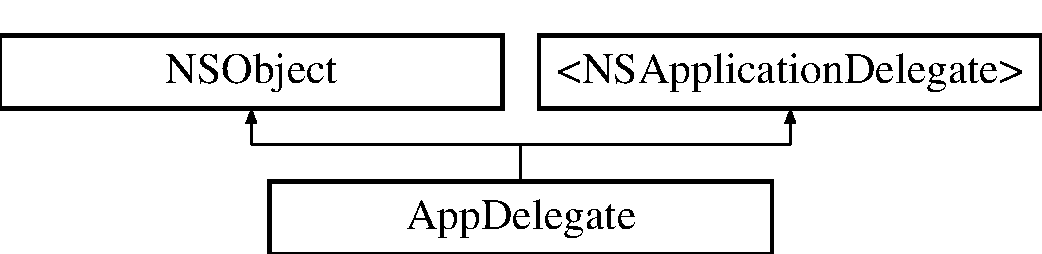
\includegraphics[height=2.000000cm]{dd/d52/interface_app_delegate}
\end{center}
\end{figure}
\subsubsection*{Instance Methods}
\begin{DoxyCompactItemize}
\item 
(void) -\/ \hyperlink{interface_app_delegate_aa03ed24826ea60753de347b0ab33adfb}{run\-Game\-Scene}
\item 
(I\-B\-Action) -\/ \hyperlink{interface_app_delegate_ae9916ea37adae8d345a8008be3aa054f}{toggle\-Full\-Screen\-:}
\end{DoxyCompactItemize}
\subsubsection*{Protected Attributes}
\begin{DoxyCompactItemize}
\item 
N\-S\-Window $\ast$ \hyperlink{interface_app_delegate_a5338c82d195ce50c948cbbf1b974665b}{window\-\_\-}
\item 
C\-C\-G\-L\-View $\ast$ \hyperlink{interface_app_delegate_a5f256d1ae550f33820c6730d70088694}{gl\-View\-\_\-}
\end{DoxyCompactItemize}
\subsubsection*{Properties}
\begin{DoxyCompactItemize}
\item 
\hypertarget{interface_app_delegate_acdf10c46711b4d6a8d95def15620afb6}{I\-B\-Outlet N\-S\-Window $\ast$ {\bfseries window}}\label{dd/d52/interface_app_delegate_acdf10c46711b4d6a8d95def15620afb6}

\item 
\hypertarget{interface_app_delegate_aa68fb87b4f494cd1f0a0ef7d55590a17}{I\-B\-Outlet C\-C\-G\-L\-View $\ast$ {\bfseries gl\-View}}\label{dd/d52/interface_app_delegate_aa68fb87b4f494cd1f0a0ef7d55590a17}

\end{DoxyCompactItemize}


\subsubsection{Detailed Description}
Application Delegate Creates app instance and binds libraries to interface builder xibs

Serves as an application wide callback object for events that affects the whole application, such as low-\/memory, etc. 

\subsubsection{Method Documentation}
\hypertarget{interface_app_delegate_aa03ed24826ea60753de347b0ab33adfb}{\index{App\-Delegate@{App\-Delegate}!run\-Game\-Scene@{run\-Game\-Scene}}
\index{run\-Game\-Scene@{run\-Game\-Scene}!AppDelegate@{App\-Delegate}}
\paragraph[{run\-Game\-Scene}]{\setlength{\rightskip}{0pt plus 5cm}-\/ (void) run\-Game\-Scene 
\begin{DoxyParamCaption}
{}
\end{DoxyParamCaption}
}}\label{dd/d52/interface_app_delegate_aa03ed24826ea60753de347b0ab33adfb}
Run\-Game\-Sceen sets up the Cocos2d environment and runs it in the application. \hypertarget{interface_app_delegate_ae9916ea37adae8d345a8008be3aa054f}{\index{App\-Delegate@{App\-Delegate}!toggle\-Full\-Screen\-:@{toggle\-Full\-Screen\-:}}
\index{toggle\-Full\-Screen\-:@{toggle\-Full\-Screen\-:}!AppDelegate@{App\-Delegate}}
\paragraph[{toggle\-Full\-Screen\-:}]{\setlength{\rightskip}{0pt plus 5cm}-\/ (I\-B\-Action) toggle\-Full\-Screen\-: 
\begin{DoxyParamCaption}
\item[{(id)}]{sender}
\end{DoxyParamCaption}
}}\label{dd/d52/interface_app_delegate_ae9916ea37adae8d345a8008be3aa054f}
Toggles from a window to full screen view point 
\begin{DoxyParams}{Parameters}
{\em sender} & is the action sending the command \\
\hline
\end{DoxyParams}
\begin{DoxyReturn}{Returns}
I\-B\-Action binding to interface builder 
\end{DoxyReturn}


\subsubsection{Member Data Documentation}
\hypertarget{interface_app_delegate_a5f256d1ae550f33820c6730d70088694}{\index{App\-Delegate@{App\-Delegate}!gl\-View\-\_\-@{gl\-View\-\_\-}}
\index{gl\-View\-\_\-@{gl\-View\-\_\-}!AppDelegate@{App\-Delegate}}
\paragraph[{gl\-View\-\_\-}]{\setlength{\rightskip}{0pt plus 5cm}-\/ (C\-C\-G\-L\-View$\ast$) gl\-View\-\_\-\hspace{0.3cm}{\ttfamily [protected]}}}\label{dd/d52/interface_app_delegate_a5f256d1ae550f33820c6730d70088694}
gl\-View is the embedded view in which cocos2d will run inside the window 

Referenced by run\-Game\-Scene.

\hypertarget{interface_app_delegate_a5338c82d195ce50c948cbbf1b974665b}{\index{App\-Delegate@{App\-Delegate}!window\-\_\-@{window\-\_\-}}
\index{window\-\_\-@{window\-\_\-}!AppDelegate@{App\-Delegate}}
\paragraph[{window\-\_\-}]{\setlength{\rightskip}{0pt plus 5cm}-\/ (N\-S\-Window$\ast$) window\-\_\-\hspace{0.3cm}{\ttfamily [protected]}}}\label{dd/d52/interface_app_delegate_a5338c82d195ce50c948cbbf1b974665b}
window is the main window to be displayed 

Referenced by run\-Game\-Scene.



The documentation for this class was generated from the following files\-:\begin{DoxyCompactItemize}
\item 
Leap\-Paint/App\-Delegate.\-h\item 
Leap\-Paint/App\-Delegate.\-m\end{DoxyCompactItemize}

\hypertarget{interface_break_out_tests}{\section{Break\-Out\-Tests Class Reference}
\label{d8/d91/interface_break_out_tests}\index{Break\-Out\-Tests@{Break\-Out\-Tests}}
}
Inheritance diagram for Break\-Out\-Tests\-:\begin{figure}[H]
\begin{center}
\leavevmode
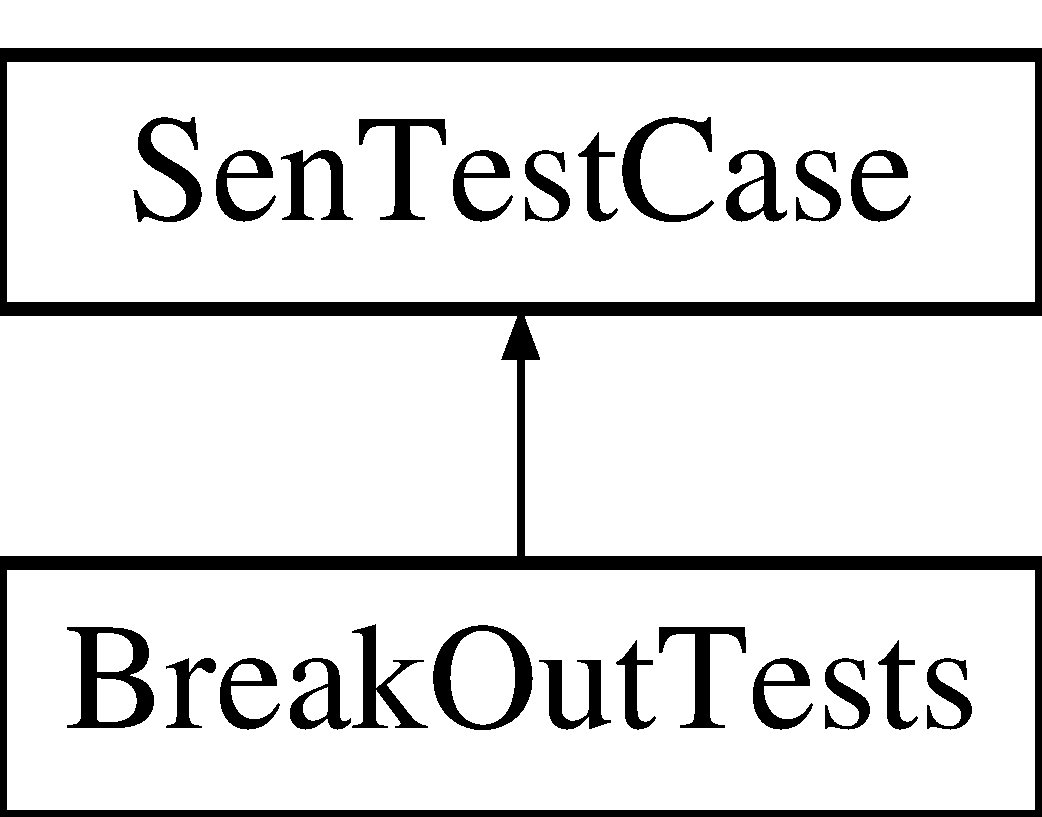
\includegraphics[height=2.000000cm]{d8/d91/interface_break_out_tests}
\end{center}
\end{figure}


\subsection{Detailed Description}


Definition at line \hyperlink{_break_out_tests_8h_source_l00011}{11} of file \hyperlink{_break_out_tests_8h_source}{Break\-Out\-Tests.\-h}.



The documentation for this class was generated from the following file\-:\begin{DoxyCompactItemize}
\item 
Break\-Out\-Tests/Break\-Out\-Tests.\-h\end{DoxyCompactItemize}

\hypertarget{class_g_l_e_s_debug_draw}{\section{G\-L\-E\-S\-Debug\-Draw Class Reference}
\label{d7/da9/class_g_l_e_s_debug_draw}\index{G\-L\-E\-S\-Debug\-Draw@{G\-L\-E\-S\-Debug\-Draw}}
}
Inheritance diagram for G\-L\-E\-S\-Debug\-Draw\-:\begin{figure}[H]
\begin{center}
\leavevmode
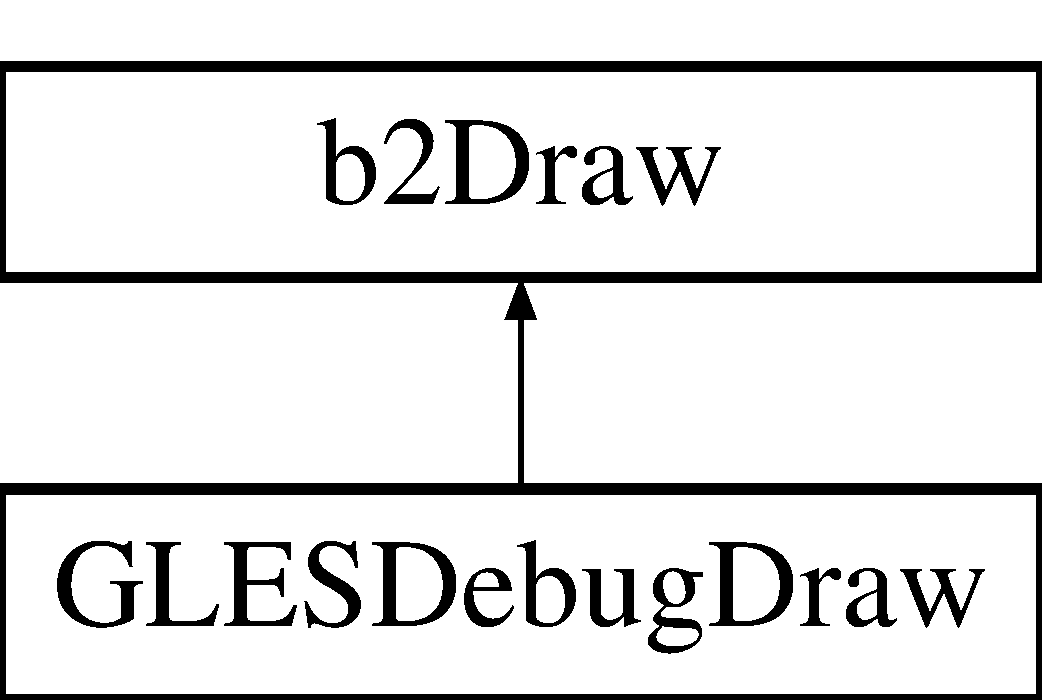
\includegraphics[height=2.000000cm]{d7/da9/class_g_l_e_s_debug_draw}
\end{center}
\end{figure}
\subsection*{Public Member Functions}
\begin{DoxyCompactItemize}
\item 
\hypertarget{class_g_l_e_s_debug_draw_a658e964ffb386b8b67fb5a3bc5db27a3}{{\bfseries G\-L\-E\-S\-Debug\-Draw} (float32 ratio)}\label{d7/da9/class_g_l_e_s_debug_draw_a658e964ffb386b8b67fb5a3bc5db27a3}

\item 
\hypertarget{class_g_l_e_s_debug_draw_afab4f8ea8882119f62134f9667e9e2da}{void {\bfseries Draw\-Polygon} (const b2\-Vec2 $\ast$vertices, int32 vertex\-Count, const b2\-Color \&color)}\label{d7/da9/class_g_l_e_s_debug_draw_afab4f8ea8882119f62134f9667e9e2da}

\item 
\hypertarget{class_g_l_e_s_debug_draw_aa68490f03cf0cb567ce6ccd78b18c5c3}{void {\bfseries Draw\-Solid\-Polygon} (const b2\-Vec2 $\ast$vertices, int32 vertex\-Count, const b2\-Color \&color)}\label{d7/da9/class_g_l_e_s_debug_draw_aa68490f03cf0cb567ce6ccd78b18c5c3}

\item 
\hypertarget{class_g_l_e_s_debug_draw_a9beacb1f221106e10ea68614ff336bf8}{void {\bfseries Draw\-Circle} (const b2\-Vec2 \&center, float32 radius, const b2\-Color \&color)}\label{d7/da9/class_g_l_e_s_debug_draw_a9beacb1f221106e10ea68614ff336bf8}

\item 
\hypertarget{class_g_l_e_s_debug_draw_ac06ea317fe6075cb9e1ff87ff89b8007}{void {\bfseries Draw\-Solid\-Circle} (const b2\-Vec2 \&center, float32 radius, const b2\-Vec2 \&axis, const b2\-Color \&color)}\label{d7/da9/class_g_l_e_s_debug_draw_ac06ea317fe6075cb9e1ff87ff89b8007}

\item 
\hypertarget{class_g_l_e_s_debug_draw_a2a24d1fe4eb99b6382380c234ab77382}{void {\bfseries Draw\-Segment} (const b2\-Vec2 \&p1, const b2\-Vec2 \&p2, const b2\-Color \&color)}\label{d7/da9/class_g_l_e_s_debug_draw_a2a24d1fe4eb99b6382380c234ab77382}

\item 
\hypertarget{class_g_l_e_s_debug_draw_a2306fb12b6f6e69d84fcb79bcddfcfbf}{void {\bfseries Draw\-Transform} (const b2\-Transform \&xf)}\label{d7/da9/class_g_l_e_s_debug_draw_a2306fb12b6f6e69d84fcb79bcddfcfbf}

\item 
\hypertarget{class_g_l_e_s_debug_draw_a84ce73b36e8b9e2843b2deacebeee839}{void {\bfseries Draw\-Point} (const b2\-Vec2 \&p, float32 size, const b2\-Color \&color)}\label{d7/da9/class_g_l_e_s_debug_draw_a84ce73b36e8b9e2843b2deacebeee839}

\item 
\hypertarget{class_g_l_e_s_debug_draw_a16aaca99009b9423fe288b5815c8dbcf}{void {\bfseries Draw\-String} (int x, int y, const char $\ast$string,...)}\label{d7/da9/class_g_l_e_s_debug_draw_a16aaca99009b9423fe288b5815c8dbcf}

\item 
\hypertarget{class_g_l_e_s_debug_draw_a6dc5d6adbc8279c9d378311b66ddcf53}{void {\bfseries Draw\-A\-A\-B\-B} (b2\-A\-A\-B\-B $\ast$aabb, const b2\-Color \&color)}\label{d7/da9/class_g_l_e_s_debug_draw_a6dc5d6adbc8279c9d378311b66ddcf53}

\end{DoxyCompactItemize}


\subsection{Detailed Description}


Definition at line \hyperlink{_g_l_e_s-_render_8h_source_l00043}{43} of file \hyperlink{_g_l_e_s-_render_8h_source}{G\-L\-E\-S-\/\-Render.\-h}.



The documentation for this class was generated from the following files\-:\begin{DoxyCompactItemize}
\item 
Leap\-Paint/G\-L\-E\-S-\/\-Render.\-h\item 
Leap\-Paint/G\-L\-E\-S-\/\-Render.\-mm\end{DoxyCompactItemize}

\hypertarget{interface_hello_world}{\section{Hello\-World Class Reference}
\label{dd/d0c/interface_hello_world}\index{Hello\-World@{Hello\-World}}
}
Inheritance diagram for Hello\-World\-:\begin{figure}[H]
\begin{center}
\leavevmode
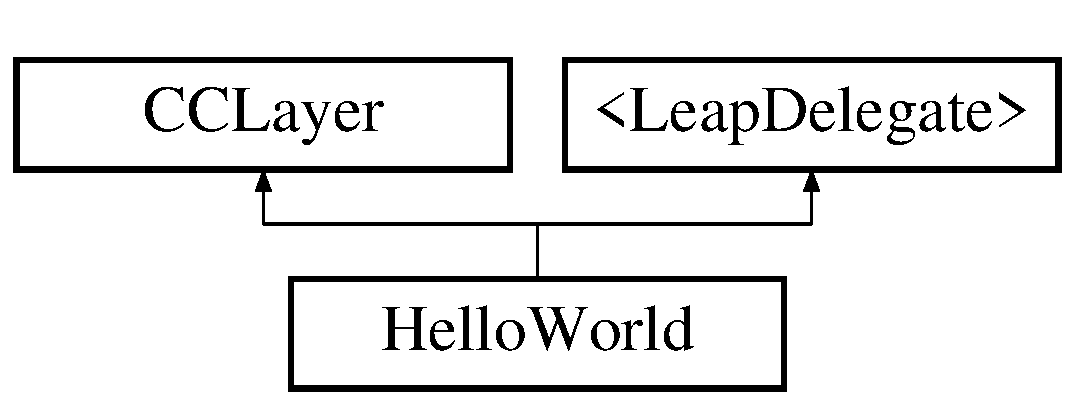
\includegraphics[height=2.000000cm]{dd/d0c/interface_hello_world}
\end{center}
\end{figure}
\subsection*{Class Methods}
\begin{DoxyCompactItemize}
\item 
\hypertarget{interface_hello_world_ad4a0819f2a6b47bd9332afe9d6007074}{(id) + {\bfseries scene}}\label{dd/d0c/interface_hello_world_ad4a0819f2a6b47bd9332afe9d6007074}

\end{DoxyCompactItemize}
\subsection*{Protected Attributes}
\begin{DoxyCompactItemize}
\item 
\hypertarget{interface_hello_world_a9723710618968a996a536bf687693185}{b2\-World $\ast$ {\bfseries \-\_\-world}}\label{dd/d0c/interface_hello_world_a9723710618968a996a536bf687693185}

\item 
\hypertarget{interface_hello_world_a70977599a3868acd441efe7088584745}{b2\-Body $\ast$ {\bfseries \-\_\-ground\-Body}}\label{dd/d0c/interface_hello_world_a70977599a3868acd441efe7088584745}

\item 
\hypertarget{interface_hello_world_af805f299cecdde22032b5b33ce812d63}{b2\-Body $\ast$ {\bfseries \-\_\-paddle\-Body}}\label{dd/d0c/interface_hello_world_af805f299cecdde22032b5b33ce812d63}

\item 
\hypertarget{interface_hello_world_aeaf675cad503a3088e045975ae0e35ba}{b2\-Fixture $\ast$ {\bfseries \-\_\-paddle\-Fixture}}\label{dd/d0c/interface_hello_world_aeaf675cad503a3088e045975ae0e35ba}

\item 
\hypertarget{interface_hello_world_acf16737495743ff9703573599bfe0c2f}{b2\-Fixture $\ast$ {\bfseries \-\_\-ball\-Fixture}}\label{dd/d0c/interface_hello_world_acf16737495743ff9703573599bfe0c2f}

\item 
\hypertarget{interface_hello_world_a8948342e97f38ccdce272b4110e67c96}{b2\-Fixture $\ast$ {\bfseries \-\_\-bottom\-Fixture}}\label{dd/d0c/interface_hello_world_a8948342e97f38ccdce272b4110e67c96}

\item 
\hypertarget{interface_hello_world_adeaa5b02c710fc36aeb98fe6528b07c0}{b2\-Mouse\-Joint $\ast$ {\bfseries \-\_\-mouse\-Joint}}\label{dd/d0c/interface_hello_world_adeaa5b02c710fc36aeb98fe6528b07c0}

\item 
\hypertarget{interface_hello_world_ab8bfb6b3e053aad4e395b654e722bf9e}{b2\-Mouse\-Joint $\ast$ {\bfseries \-\_\-finger\-Joint}}\label{dd/d0c/interface_hello_world_ab8bfb6b3e053aad4e395b654e722bf9e}

\item 
\hypertarget{interface_hello_world_a6d39f287d5cb57fb6f117d07112f823c}{My\-Contact\-Listener $\ast$ {\bfseries \-\_\-contact\-Listener}}\label{dd/d0c/interface_hello_world_a6d39f287d5cb57fb6f117d07112f823c}

\item 
\hypertarget{interface_hello_world_af12f83384b70d9d5cbea1d3e72be5443}{Leap\-Controller $\ast$ {\bfseries controller}}\label{dd/d0c/interface_hello_world_af12f83384b70d9d5cbea1d3e72be5443}

\item 
\hypertarget{interface_hello_world_a797f5dc66315291bb60d2d2876a9d10b}{N\-S\-Mutable\-Dictionary $\ast$ {\bfseries trackable\-List}}\label{dd/d0c/interface_hello_world_a797f5dc66315291bb60d2d2876a9d10b}

\item 
\hypertarget{interface_hello_world_a2c25ec48f85d3df5ea629537feab7262}{B\-O\-O\-L {\bfseries finger\-Tracked}}\label{dd/d0c/interface_hello_world_a2c25ec48f85d3df5ea629537feab7262}

\end{DoxyCompactItemize}


\subsection{Detailed Description}


Definition at line \hyperlink{_hello_world_scene_8h_source_l00012}{12} of file \hyperlink{_hello_world_scene_8h_source}{Hello\-World\-Scene.\-h}.



The documentation for this class was generated from the following files\-:\begin{DoxyCompactItemize}
\item 
Break\-Out/Hello\-World\-Scene.\-h\item 
Break\-Out/Hello\-World\-Scene.\-mm\end{DoxyCompactItemize}

\hypertarget{interface_hello_world_layer}{\section{Hello\-World\-Layer Class Reference}
\label{dd/d46/interface_hello_world_layer}\index{Hello\-World\-Layer@{Hello\-World\-Layer}}
}
Inheritance diagram for Hello\-World\-Layer\-:\begin{figure}[H]
\begin{center}
\leavevmode
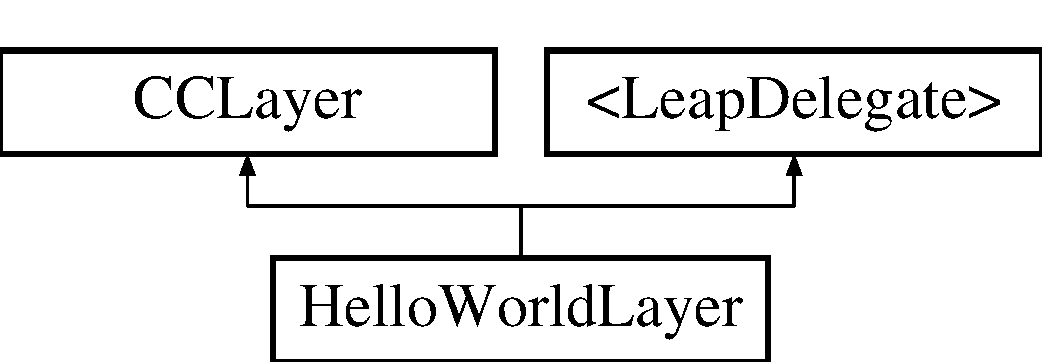
\includegraphics[height=2.000000cm]{dd/d46/interface_hello_world_layer}
\end{center}
\end{figure}
\subsection*{Protected Attributes}
\begin{DoxyCompactItemize}
\item 
\hypertarget{interface_hello_world_layer_a26559878fa538b7643e833bd9cc1b1e7}{Leap\-Controller $\ast$ {\bfseries controller}}\label{dd/d46/interface_hello_world_layer_a26559878fa538b7643e833bd9cc1b1e7}

\item 
\hypertarget{interface_hello_world_layer_a7e0ef6411af9a35a21203b2c9da461c2}{C\-C\-Texture2\-D $\ast$ {\bfseries sprite\-Texture\-\_\-}}\label{dd/d46/interface_hello_world_layer_a7e0ef6411af9a35a21203b2c9da461c2}

\item 
\hypertarget{interface_hello_world_layer_adec36773d5e2f9d49fa589a6ea9bfbd0}{b2\-World $\ast$ {\bfseries world}}\label{dd/d46/interface_hello_world_layer_adec36773d5e2f9d49fa589a6ea9bfbd0}

\item 
\hypertarget{interface_hello_world_layer_a311e7dc2cec43a99d9ef757a2a2fcf0d}{\hyperlink{class_g_l_e_s_debug_draw}{G\-L\-E\-S\-Debug\-Draw} $\ast$ {\bfseries m\-\_\-debug\-Draw}}\label{dd/d46/interface_hello_world_layer_a311e7dc2cec43a99d9ef757a2a2fcf0d}

\item 
\hypertarget{interface_hello_world_layer_a8f48c2997a2f55dc1a1377ed07c812d8}{C\-C\-Sprite $\ast$ {\bfseries target\-Sprite}}\label{dd/d46/interface_hello_world_layer_a8f48c2997a2f55dc1a1377ed07c812d8}

\item 
\hypertarget{interface_hello_world_layer_a1c838da6242937b18d9f51b19ac76b11}{b2\-Mouse\-Joint $\ast$ {\bfseries \-\_\-mouse\-Joint}}\label{dd/d46/interface_hello_world_layer_a1c838da6242937b18d9f51b19ac76b11}

\item 
\hypertarget{interface_hello_world_layer_ab173e766b18c692bb4358fa84b40aca4}{b2\-World $\ast$ {\bfseries \-\_\-world}}\label{dd/d46/interface_hello_world_layer_ab173e766b18c692bb4358fa84b40aca4}

\item 
\hypertarget{interface_hello_world_layer_a70af821707c84fe8a933578576d1e9b1}{b2\-Body $\ast$ {\bfseries \-\_\-ground\-Body}}\label{dd/d46/interface_hello_world_layer_a70af821707c84fe8a933578576d1e9b1}

\item 
\hypertarget{interface_hello_world_layer_af526e0952720a2778df5cdceb69227c1}{N\-S\-Mutable\-Dictionary $\ast$ {\bfseries trackable\-List}}\label{dd/d46/interface_hello_world_layer_af526e0952720a2778df5cdceb69227c1}

\end{DoxyCompactItemize}


\subsection{Detailed Description}


Definition at line \hyperlink{_hello_world_layer_8h_source_l00018}{18} of file \hyperlink{_hello_world_layer_8h_source}{Hello\-World\-Layer.\-h}.



The documentation for this class was generated from the following file\-:\begin{DoxyCompactItemize}
\item 
Break\-Out/Hello\-World\-Layer.\-h\end{DoxyCompactItemize}

\hypertarget{category_hello_world_layer_07_08}{\section{Hello\-World\-Layer() Category Reference}
\label{d1/d30/category_hello_world_layer_07_08}\index{Hello\-World\-Layer()@{Hello\-World\-Layer()}}
}
\subsection*{Instance Methods}
\begin{DoxyCompactItemize}
\item 
\hypertarget{category_hello_world_layer_07_08_ab3500df9c05677d31170bcb07a82f522}{(void) -\/ {\bfseries init\-Physics}}\label{d1/d30/category_hello_world_layer_07_08_ab3500df9c05677d31170bcb07a82f522}

\item 
\hypertarget{category_hello_world_layer_07_08_a1d9f76267b1dabaa3f25f7530ef0b062}{(void) -\/ {\bfseries add\-New\-Sprite\-At\-Position\-:}}\label{d1/d30/category_hello_world_layer_07_08_a1d9f76267b1dabaa3f25f7530ef0b062}

\item 
\hypertarget{category_hello_world_layer_07_08_a816e77da1323550bd1bb9ad89354dec1}{(void) -\/ {\bfseries create\-Reset\-Button}}\label{d1/d30/category_hello_world_layer_07_08_a816e77da1323550bd1bb9ad89354dec1}

\end{DoxyCompactItemize}


\subsection{Detailed Description}


Definition at line \hyperlink{_hello_world_layer_8mm_source_l00026}{26} of file \hyperlink{_hello_world_layer_8mm_source}{Hello\-World\-Layer.\-mm}.



The documentation for this category was generated from the following file\-:\begin{DoxyCompactItemize}
\item 
Break\-Out/Hello\-World\-Layer.\-mm\end{DoxyCompactItemize}

\hypertarget{interface_physics_sprite}{\section{Physics\-Sprite Class Reference}
\label{db/d8a/interface_physics_sprite}\index{Physics\-Sprite@{Physics\-Sprite}}
}
Inheritance diagram for Physics\-Sprite\-:\begin{figure}[H]
\begin{center}
\leavevmode
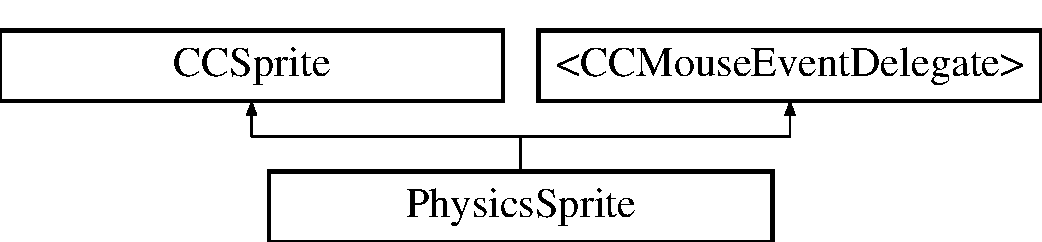
\includegraphics[height=2.000000cm]{db/d8a/interface_physics_sprite}
\end{center}
\end{figure}
\subsection*{Instance Methods}
\begin{DoxyCompactItemize}
\item 
\hypertarget{interface_physics_sprite_a853b9462e896123262409338f932b76a}{(void) -\/ {\bfseries set\-Physics\-Body\-:}}\label{db/d8a/interface_physics_sprite_a853b9462e896123262409338f932b76a}

\item 
\hypertarget{interface_physics_sprite_a1a663e8f4b61843f86825acf96ea49da}{(void) -\/ {\bfseries set\-Target\-:}}\label{db/d8a/interface_physics_sprite_a1a663e8f4b61843f86825acf96ea49da}

\item 
\hypertarget{interface_physics_sprite_a7f7f8bd12fb3436017b2ee2ee83d679b}{(void) -\/ {\bfseries del\-Target}}\label{db/d8a/interface_physics_sprite_a7f7f8bd12fb3436017b2ee2ee83d679b}

\end{DoxyCompactItemize}
\subsection*{Protected Attributes}
\begin{DoxyCompactItemize}
\item 
\hypertarget{interface_physics_sprite_aa94b7391bdfa00bc0d4c3dc8e9141513}{C\-G\-Point {\bfseries target}}\label{db/d8a/interface_physics_sprite_aa94b7391bdfa00bc0d4c3dc8e9141513}

\item 
\hypertarget{interface_physics_sprite_a038f4e8bdc36d8a71fdbdd34a85c61b7}{uint {\bfseries ticker}}\label{db/d8a/interface_physics_sprite_a038f4e8bdc36d8a71fdbdd34a85c61b7}

\item 
\hypertarget{interface_physics_sprite_ac9cf5f072dbf14242a89a44a85243023}{bool {\bfseries has\-Target}}\label{db/d8a/interface_physics_sprite_ac9cf5f072dbf14242a89a44a85243023}

\item 
\hypertarget{interface_physics_sprite_af07493ad48010e6bf4bd31389c724e9f}{b2\-Body $\ast$ {\bfseries body\-\_\-}}\label{db/d8a/interface_physics_sprite_af07493ad48010e6bf4bd31389c724e9f}

\end{DoxyCompactItemize}


\subsection{Detailed Description}


Definition at line \hyperlink{_physics_sprite_8h_source_l00016}{16} of file \hyperlink{_physics_sprite_8h_source}{Physics\-Sprite.\-h}.



The documentation for this class was generated from the following files\-:\begin{DoxyCompactItemize}
\item 
Break\-Out/Physics\-Sprite.\-h\item 
Break\-Out/Physics\-Sprite.\-mm\end{DoxyCompactItemize}

\hypertarget{interface_pong_scene}{\section{Pong\-Scene Class Reference}
\label{d4/d8f/interface_pong_scene}\index{Pong\-Scene@{Pong\-Scene}}
}
Inheritance diagram for Pong\-Scene\-:\begin{figure}[H]
\begin{center}
\leavevmode
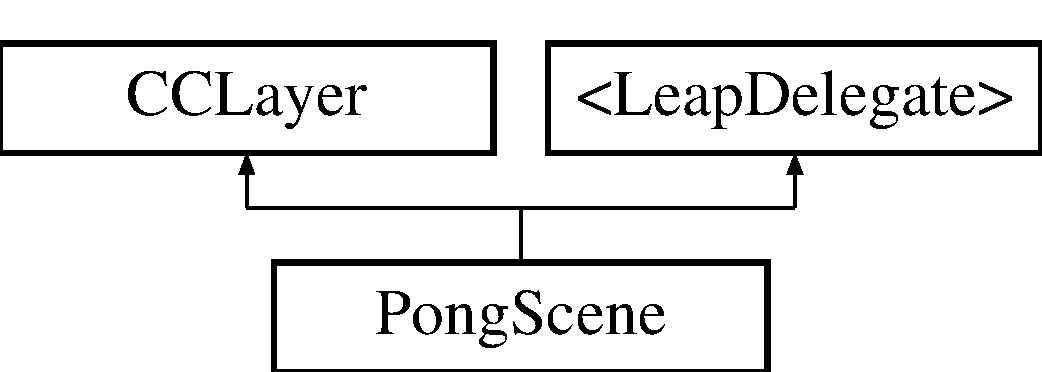
\includegraphics[height=2.000000cm]{d4/d8f/interface_pong_scene}
\end{center}
\end{figure}
\subsection*{Protected Attributes}
\begin{DoxyCompactItemize}
\item 
\hypertarget{interface_pong_scene_a275744db48056c5611403ef4fcc42146}{Leap\-Controller $\ast$ {\bfseries controller}}\label{d4/d8f/interface_pong_scene_a275744db48056c5611403ef4fcc42146}

\item 
\hypertarget{interface_pong_scene_a528d5af5fd4a49fb36babb03092a4666}{C\-C\-Texture2\-D $\ast$ {\bfseries sprite\-Texture\-\_\-}}\label{d4/d8f/interface_pong_scene_a528d5af5fd4a49fb36babb03092a4666}

\item 
\hypertarget{interface_pong_scene_a090f93c97c398e1d0f3b98a595ffd474}{b2\-World $\ast$ {\bfseries world}}\label{d4/d8f/interface_pong_scene_a090f93c97c398e1d0f3b98a595ffd474}

\item 
\hypertarget{interface_pong_scene_a6c160ce6b62c51559fe1f19ec41481a5}{\hyperlink{class_g_l_e_s_debug_draw}{G\-L\-E\-S\-Debug\-Draw} $\ast$ {\bfseries m\-\_\-debug\-Draw}}\label{d4/d8f/interface_pong_scene_a6c160ce6b62c51559fe1f19ec41481a5}

\item 
\hypertarget{interface_pong_scene_ae2be6151855e73d2fd2fd3408aa3a82d}{C\-C\-Sprite $\ast$ {\bfseries target\-Sprite}}\label{d4/d8f/interface_pong_scene_ae2be6151855e73d2fd2fd3408aa3a82d}

\item 
\hypertarget{interface_pong_scene_ab26c034621823c35b14832559bf79b92}{b2\-Mouse\-Joint $\ast$ {\bfseries \-\_\-mouse\-Joint}}\label{d4/d8f/interface_pong_scene_ab26c034621823c35b14832559bf79b92}

\item 
\hypertarget{interface_pong_scene_a1fcc0b15bb8f532f9d031b901750a856}{b2\-World $\ast$ {\bfseries \-\_\-world}}\label{d4/d8f/interface_pong_scene_a1fcc0b15bb8f532f9d031b901750a856}

\item 
\hypertarget{interface_pong_scene_afe1a93d7fb8e281d9631a5587879d773}{b2\-Body $\ast$ {\bfseries \-\_\-ground\-Body}}\label{d4/d8f/interface_pong_scene_afe1a93d7fb8e281d9631a5587879d773}

\item 
\hypertarget{interface_pong_scene_a1cb88a8020e379a68fd3305324aeeb8c}{N\-S\-Mutable\-Dictionary $\ast$ {\bfseries trackable\-List}}\label{d4/d8f/interface_pong_scene_a1cb88a8020e379a68fd3305324aeeb8c}

\end{DoxyCompactItemize}


\subsection{Detailed Description}


Definition at line \hyperlink{_pong_scene_8h_source_l00015}{15} of file \hyperlink{_pong_scene_8h_source}{Pong\-Scene.\-h}.



The documentation for this class was generated from the following file\-:\begin{DoxyCompactItemize}
\item 
Break\-Out/Pong\-Scene.\-h\end{DoxyCompactItemize}

\addcontentsline{toc}{part}{Index}
\printindex
\end{document}
